\documentclass{beamer}	
\usepackage{color}
\usepackage{parskip}
\usepackage{graphicx}
\usepackage{multirow}
\usepackage{listings}
\usepackage{amsmath}
\usepackage{amssymb}
\definecolor{mygreen}{rgb}{0,0.6,0}
\definecolor{lbcolor}{rgb}{0.9,0.9,0.9}


\usetheme{Madrid}

\title{The PH-Tree: A Space-Efficient Storage Structure and Multi-Dimensional Index}

\author{Christofer Fabian Chavez Carazas}

\institute{National University of Saint Augustine}

\date{\today}

\lstset{
backgroundcolor=\color{lbcolor},
    tabsize=4,    
%   rulecolor=,
    language=[GNU]C++,
        basicstyle=\tiny,
        aboveskip={1.5\baselineskip},
        columns=fixed,
        showstringspaces=false,
        extendedchars=false,
        breaklines=true,
        prebreak = \raisebox{0ex}[0ex][0ex]{\ensuremath{\hookleftarrow}},
        frame=single,
        showtabs=false,
        showspaces=false,
        showstringspaces=false,
        identifierstyle=\ttfamily,
        keywordstyle=\color[rgb]{0,0,1},
        commentstyle=\color[rgb]{0.026,0.112,0.095},
        stringstyle=\color{red},
        numberstyle=\color[rgb]{0.205, 0.142, 0.73},
%        \lstdefinestyle{C++}{language=C++,style=numbers}’.
}

\begin{document}
 
 \begin{frame}
  \titlepage
 \end{frame}

\begin{frame}{Introduction}
  \begin{block}{}
    PATRICIA-hypercube-tree
   \end{block}
  \begin{block}{}
   Efficient data access.
  \end{block}
  \begin{block}{}
   Space efficiency
  \end{block}
  \begin{block}{}
   Compare to kd-tree
  \end{block}
\end{frame}

\begin{frame}{Bit-stream}
  \begin{itemize}
    \item The bit stream is the representation of the data in each dimension using bits.
  \end{itemize}
  \begin{block}{Example}
   1D Example: \\
   \begin{center}
      10 to binary: 1010  \\
      Bit-stream: 1 0 1 0
   \end{center}
   2D Example: \\
   \begin{center}
      (10,5) to binary: (1010,0101) \\
      Bit-stream: 10 01 10 01
   \end{center}
   3D Example: \\
   \begin{center}
      (4,8,1) to binary: (0100,1000,0001) \\
      Bit-stream: 010 100 000 001
   \end{center}
  \end{block}
  \begin{itemize}
   \item $w$ is the size of the bit-stream and the depth of the PH-Tree.
  \end{itemize}
\end{frame}

\begin{frame}{Prefix Sharing (PATRICIA-Trie)}
 \begin{figure}[h]
  \centering
  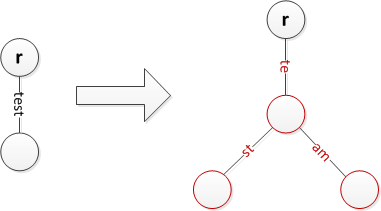
\includegraphics[scale = 0.3]{2.png}
  \label{fig2}
  \caption{Insert ``test'' and later insert ``team''}
 \end{figure}

 \begin{figure}[h]
  \centering
  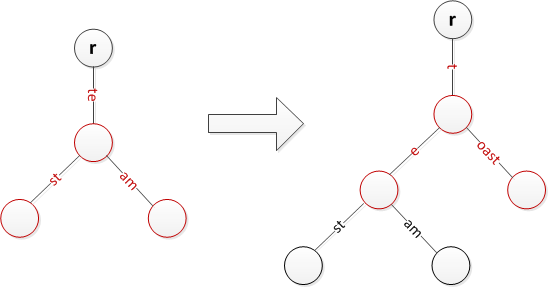
\includegraphics[scale = 0.3]{3.png}
  \label{fig3}
  \caption{Insert ``toast''}
 \end{figure}
\end{frame}


\begin{frame}{PH-Tree - Structure}
   \begin{figure}[h]
    \centering
    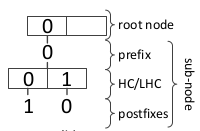
\includegraphics[scale=0.5]{1.png}
    \label{fig1}
    \caption{PH-Tree Structure}
  \end{figure}
  \begin{block}{One node have:}
    \begin{itemize}
     \item Prefix
     \item Hypercube
     \item Postfixes or sub-nodes
    \end{itemize}
  \end{block}

\end{frame}

\begin{frame}{Hypercube}
  \begin{itemize}
   \item The hypercubes allows navigation to subnodes and postfixes.
  \end{itemize}
  \begin{figure}
   \centering
   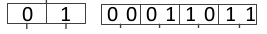
\includegraphics[scale = 0.7]{4.png}
   \label{fig4}
   \caption{1D and 2D Hypercubes}
  \end{figure}
  \begin{itemize}
   \item The size of the hypercube is $2^{k}$.
  \end{itemize}
\end{frame}

\begin{frame}{Insert}
 \begin{itemize}
  \item We insert the point (5,9) : (0101,1001)
 \end{itemize}
 
 \begin{figure}
   \centering
   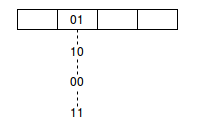
\includegraphics{5.png}
   \label{fig5}
   \caption{First insertion}
 \end{figure}
\end{frame}


\begin{frame}{Insert}
  \begin{itemize}
   \item We insert the point (6,10) : (0110,1010)
  \end{itemize}
  
  \begin{figure}
   \centering
   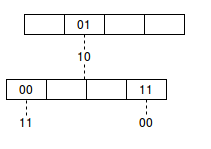
\includegraphics{6.png}
   \label{fig6}
   \caption{Second insertion}
  \end{figure}
\end{frame}

\begin{frame}{Insert}
 \begin{itemize}
  \item We insert the point (6,8) : (0110,1000)
 \end{itemize}
 
 \begin{figure}
  \centering
  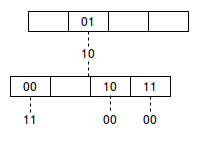
\includegraphics{7.png}
  \label{fig7}
  \caption{Third insertion}
 \end{figure}
\end{frame}

\begin{frame}{HC/LHC}
 \begin{itemize}
  \item \textbf{HC (HiperCube):} An Array of references.
  \item \textbf{LHC (Linear HiperCube:} An a list of pairs that map \\ $<$address in HC$>$ -$>$ $<$postfix/sub-node$>$
 \end{itemize}

 \begin{figure}
  \centering
  
\includegraphics[scale = 0.5]{8.png}
  \label{fig8}
  \caption{HC (left) and LHC (right) representation of hypercube (top) in a node}
 \end{figure}

\end{frame}

\begin{frame}{HC/LHC}
\begin{block}{Advantages and Disadvantages:}
 \begin{itemize}
  \item \textbf{HC:} It requires only constant time operation to navigate to the sub-node or stored entry, but it wastes space.
  \item \textbf{LHC:} It saves up space, but it requires a binary search to navigate to the sub-node or stored entry.
 \end{itemize}
\end{block}
 \begin{block}{Calculating the Space}
  \begin{itemize}
   \item \textbf{HC:} $O(2^{k})$ for the sub-nodes and $O(l_{p} * 2^{k})$ for the postfixes
   \item \textbf{LHC:} $O(n_{s} * k)$ for the sub-nodes and $O(n_{p} * k * l_{p})$ for the postfixes.
  \end{itemize}
  Where:
  \begin{itemize}
   \item $k$ is the number of dimensions.
   \item $l_{p}$ is the length of the postfixes in a node.
   \item $n_{s}$ is the number of sub-nodes.
   \item $n_{p}$ is the number of posfixes.
  \end{itemize}
 \end{block}
\end{frame}

\begin{frame}{Point Query}
  Search the point (10,8) : (1010,1000). \\
  Bit-stream: 11 00 10 00 \par
  
  Search the point (1,1) : (0001,0001) \\
  Bit-stream: 00 00 00 11

  \begin{figure}
   \centering
   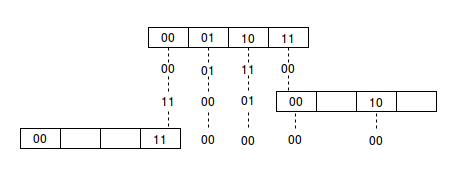
\includegraphics[scale = 0.5]{9.png}
   \label{fig9}
   \caption{PH-tree example}
  \end{figure}
\end{frame}


\begin{frame}{Range Query}
  \begin{itemize}
   \item Input: lower left point and uper rigth point.
   \item Output: Iterator.
  \end{itemize}
  \begin{enumerate}
   \item Start with a point query that locates the starting node, defined as the lower left corner of the query range. Even if the point query fails, the last visited node
    is the starting point for the query.
   \item Calculate two bit masks $m_{L}$ and $m_{U}$
   \begin{enumerate}
    \item $m_{L}$ is set to 0 if the query range is less or equal to the lower left corner of the node in the dimension $i$.
    \item Inversely, any bit b i in $m_{U}$ is set to 1 if the query range is equal to or larger than the top right corner of the node.
   \end{enumerate}
   \item An HC address h fits if $(h|m_{L})$ $==$ $h$ $\&\&$ $(h\&m_{U})$ $==$ $h$
   \item Continue iterating until there are not candidates.
   \item If the candidate is a node, then repeat the step two.
  \end{enumerate}
\end{frame}

\begin{frame}{Space Efficiency}
 \begin{block}{Worst Cases}
   \begin{itemize}
    \item Lack of prefix sharing. \textbf{HC:}$O(w * 2^{k})$  \textbf{LHC:}$O(w * k * n)$
    \item Bad entry to node ratio     ($r_{e/n} = n/n_{node}$)
   \end{itemize}
 \end{block}
 \begin{figure}
  \centering
  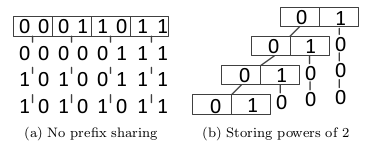
\includegraphics[scale = 0.5]{11.png}
  \label{fig11}
  \caption{The two space worst cases of the PH-Tree}
 \end{figure}

 \begin{itemize}  
 \item The average case cannot be established as a simple function of n because it not only depends on the type of distribution of the data but also on the value range in each dimension.
 \end{itemize}
 
\end{frame}

\begin{frame}{Query Efficiency}
 \begin{block}{Point Query}
 \begin{itemize}
  \item Algorithm for interleaving: $O(w*k)$
  \item Query internal search: \textbf{HC:} $O(1)$ \textbf{LHC:} $O(log_{2}(2^{k})) = O(k)$
  \item Prefix/postfix extraction: $O(w*k)$
  \item Putting everything together: \textbf{HC:} $O(w*k + w*1 + w*k)$ \textbf{LHC:} $O(w*k + w * log k + w * k)$
  \item Resulting $O(w*k)$ for both approaches.
 \end{itemize}
 \end{block}
 
 \begin{block}{Range Query}
  \begin{itemize}
   \item The worst case is a full scan of the nodes with $O(n)$
  \end{itemize}
 \end{block}
 
 \begin{itemize}
  \item The average complexity cannot be established as a simple function of n, because it depends on different characteristics of the data.
  \item The query complexity tends to vary between $O(log n)$ and $O(1)$  for low $w$
 \end{itemize}
\end{frame}

\begin{frame}{Update Efficiency}
  \begin{itemize}
    \item Point query: $O(w * k)$
    \item Creation of sub-node: $O(1)$
    \item Encoding the new entry and copying an existing postfix from the parent node: $O(w*k)$
    \item Insert in the LHC: $O(w * 2^k)$
    \item Insert in the HC: $O(1)$
    \item Total cost of the LHC: $O(w * (2^k + k))$
    \item Total cost of the HC: $O(w * k)$
  \end{itemize}
\end{frame}

\begin{frame}{Experiment}
 \begin{block}{Set-Up}
  \begin{itemize}
   \item PC with 32GB RAM and and Intel i7-3770K 3.50GHz GPU.
   \item They used two kD-tree implementations called KD1 and KD2.
   \item They used two critical-bit-trees(bit-wise PATRICIA-tries) called CB1 and CB2.
  \end{itemize}
 \end{block}
 \begin{block}{Datasets}
  \begin{itemize}
   \item \textbf{2D TIGER/Line:} It consists of poly-lines that describe map features of the United States of America. They extracted all points from counties belonging to mainland USA. $18.4 * 10^6$
   \item \textbf{3D CUBE:} is a set of up to 100,000,000 points distributed uni-formly at random between 0.0 and 1.0 and independently in every dimension.
   \item \textbf{3D CLUSTER:} The dataset consists of a line of 10000 evenly spaced clusters of points. In total, the CLUSTER dataset contains up to 50,000,000 points.
  \end{itemize}
 \end{block}
\end{frame}

\begin{frame}{Experiment}
 \begin{figure}
  \centering
  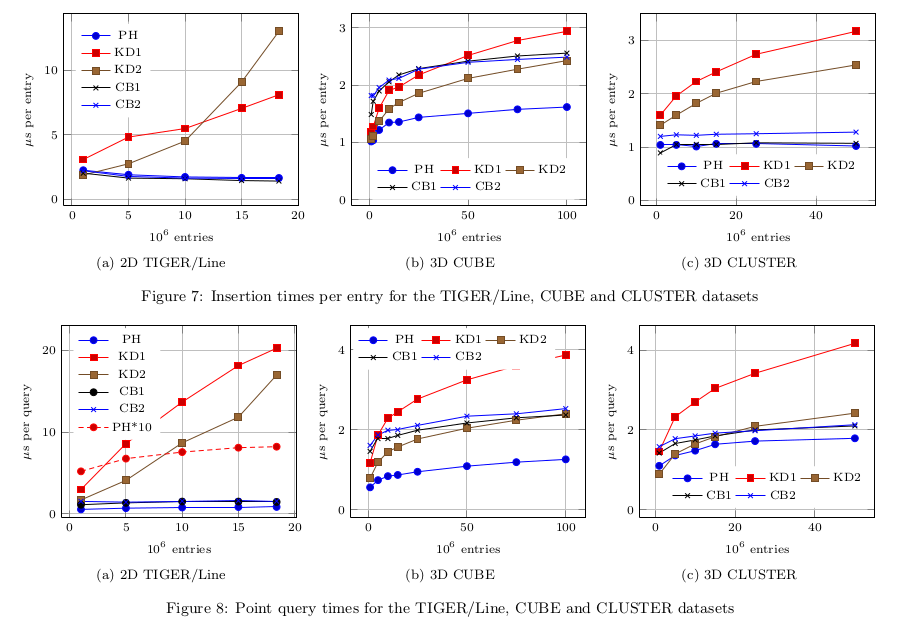
\includegraphics[scale = 0.3]{12.png}
 \end{figure}
\end{frame}

\begin{frame}{Experiment}
 \begin{figure}
  \centering
  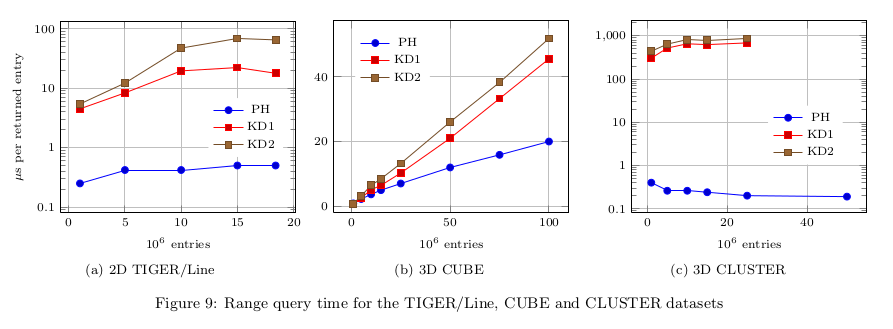
\includegraphics[scale = 0.35]{13.png}
 \end{figure}
\end{frame}

\begin{frame}{Bibliografía}
  \begin{thebibliography}{10}
  \beamertemplatebookbibitems
    \bibitem{Libro}
    Tilmann Zäschke, Christoph Zimmerli, and Moira C. Norrie. 2014.
    \newblock The PH-tree: a space-efficient storage structure and multi-dimensional index.\par
    In Proceedings of the 2014 ACM SIGMOD International Conference on Management of Data (SIGMOD '14).
    \newblock ACM, New York, NY, USA, 397-408.
    \newblock DOI: http://dx.doi.org/10.1145/2588555.2588564 
   \end{thebibliography}
\end{frame}
 
\end{document}
